\documentclass[11pt]{standalone}

\usepackage{helvet}

\usepackage{ifthen}
\usepackage{tikz} 
\usetikzlibrary{shapes.misc}
\usetikzlibrary{arrows,arrows.meta}
\usetikzlibrary{calc,intersections, patterns, math}

\definecolor{pfeil}{RGB}{168,167,167}
\definecolor{petrol}{RGB}{0, 118, 136}
\definecolor{darkgoldenrod}{RGB}{184, 134, 11}
\colorlet{petrol-lighter}{petrol!40}
\colorlet{darkgoldenrod-lighter}{darkgoldenrod!40}

\begin{document}

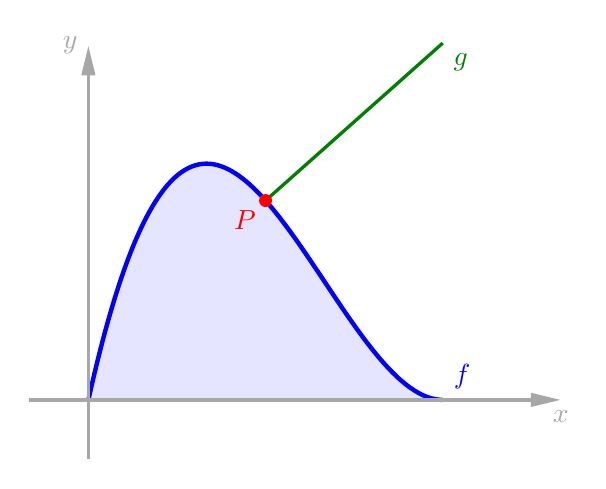
\begin{tikzpicture}[pfeil, scale=1.5,>={Triangle[length=0pt 9,width=0pt 4]}]

    % \draw[thick, fill=petrol!20, draw=petrol-lighter, rounded corners=2ex, opacity=0.5] (0,0) rectangle ++ (1.5,3.5);
    % \draw[thick, fill=darkgoldenrod!20, draw=darkgoldenrod-lighter, rounded corners=2ex, opacity=0.5] (5,0) rectangle ++ (1.5,3.5);

		
		\draw[blue, ultra thick, smooth, domain=0:3, samples = 100, fill=blue!10] plot(\x,{1/2*\x^3-3*\x^2+9/2*\x}) node[above right]{$f$};		
		\draw[green!50!black, very thick] (1.5,1.6875) --++ (1.5,1.5*8/9) node[below right] {$g$};
		\draw[fill, red] (1.5,1.6875) circle (0.05) node[below left] {$P$};
		
		\draw[very thick, ->] (-0.5,0) -- (4,0) node [below] {$x$};
		\draw[very thick, ->] (0,-0.5) -- (0,3) node[left] {$y$};
		 
    

\end{tikzpicture}

\end{document}
